\documentclass{ximera}

\input{../preamble.tex}

\outcome{Compute derivatives of polar curves.}
\outcome{Determine where the derivative of a polar curve is undefined.}
\outcome{Find the equation of a tangent lines to a polar curve.}

\title[Dig-In:]{Derivatives of polar functions}

\begin{document}
\begin{abstract}
  We differentiate polar functions.
\end{abstract}
\maketitle

The previous section discussed a special class of parametic functions,
polar functions.  We know that
\begin{align*}
  \d x &= x'(t) \d t\\
  \d y &= y'(t) \d t,
\end{align*}
and so we can compute the derivative of $y$ with respect to $x$ using
differentials:
\[
\frac{\d y}{\d x} = \frac{y'(t) \d t}{x'(t) \d t} = \frac{y'(t)}{x'(t)}
\]
provided that $x'(t) \ne 0$.  With polar functions we have
\begin{align*}
  x(\theta) &= r(\theta) \cdot \cos(\theta)\\
  y(\theta) &= r(\theta) \cdot \sin(\theta),
\end{align*}
so
\begin{align*}
\dd[y]{x} &= \frac{y'(\theta)}{x'(\theta)} \\
&= \frac{r'(\theta)\sin(\theta)+r(\theta)\cos(\theta)}{r'(\theta)\cos(\theta)-r(\theta)\sin(\theta)}
\end{align*}
provided that $x'(\theta)\ne 0$.

\begin{example}
  Consider the lima\c con $r(\theta) =1+2\sin(\theta)$ on $[0,2\pi]$
  \begin{image}
     \begin{tikzpicture}
          \begin{polaraxis}[
              xtick={0,45,...,360},
              xticklabels={$0$,$\frac{\pi}{4}$,$\frac{\pi}{2}$,$\frac{3\pi}{4}$,$\pi$,$\frac{5\pi}{4}$,$\frac{3\pi}{2}$,$\frac{7\pi}{4}$,$2\pi$},
            ]
            \addplot+[very thick, mark=none,penColor,domain=0:360,samples=100,smooth] {1+2*sin(x)};
          \end{polaraxis}
     \end{tikzpicture}
  \end{image}
  Find the equation of the tangent line to the curve at
  $\theta=\pi/4$.
  \begin{explanation}
    We start by computing the derivative in rectanglar coordinates. Recall that
    \begin{align*}
      x(\theta) &= \left(1+2\sin(\theta)\right)\cdot \cos(\theta) = \cos(\theta)+2\sin(\theta)\cos(\theta)\\
      y(\theta) &= \left(1+2\sin(\theta)\right)\cdot \sin(\theta) = \sin(\theta)+2\sin^2(\theta)
    \end{align*}
    \[
    \dd[y]{x} = \frac{\cos(\theta) + 4\sin(\theta)\cos(\theta)}{-\sin(\theta) + 2\cos^2(\theta)-2\sin^2(\theta)}
    \]
    When $\theta=\pi/4$,
    \begin{align*}
      x(\theta) &= \answer[given]{1+\sqrt{2}/2}\\
      y(\theta) &=\answer[given]{1+\sqrt{2}/2}\\
    \frac{dy}{dx} &=\answer[given]{-2\sqrt{2}-1}
    \end{align*}
     Thus the rectangular equation of the line tangent to the lima\c con at $\theta=\pi/4$ is
    \[
    y=(-2\sqrt{2}-1)\big(x-(1+\sqrt{2}/2)\big)+1+\sqrt{2}/2 \approx  -3.83 x+8.24.
    \]
    \begin{prompt}
      \graph{r=1+2\sin(\theta), y=(-2\sqrt{2}-1)(x-(1+\sqrt{2}/2))+1+\sqrt{2}/2}
    \end{prompt}
  \end{explanation}
\end{example}





\begin{example}
Find Cartesian coordinates for where the graph of $r(\theta)
=1+2\sin(\theta)$ on $[0,2\pi]$ has horizontal tangent lines.
\begin{explanation}
  To find the horizontal tangent lines, we find where $\dd[y]{x}=0$.
  Since
  \[
  \dd[y]{x} =\frac{\cos(\theta) + 4\sin(\theta)\cos(\theta)}{-\sin(\theta) + 2\cos^2(\theta)-2\sin^2(\theta)}
  \]
  we must find where the numerator is $0$. Since the numerator is equal to
  \[
  \cos(\theta)(1+ 4\sin(\theta))
  \]
  the numerator is zero when 
  \begin{itemize}
  \item $\cos(\theta)=0$ or
  \item $1+4\sin(\theta)=0$.
  \end{itemize}
  On $[0,2\pi]$, $\cos(\theta)=0$ when
  \begin{itemize}
  \item $\theta=\pi/2$ or
  \item $\theta= 3\pi/2$.
  \end{itemize}
  This cooresponds to the points
  \begin{align*}
    x(\pi/2) &= \left(1+2\sin(\pi/2)\right)\cdot\cos(\pi/2)\\
    &= 0,\\
    y(\pi/2) &= \left(1+2\sin(\pi/2)\right)\cdot\sin(\pi/2)\\
    &= 3,
  \end{align*}
  meaning $(x,y) = (0,3)$, and
  \begin{align*}
    x(3\pi/2) &= \left(1+2\sin(3\pi/2)\right)\cdot\cos(3\pi/2)\\
    &= 0,\\
    y(3\pi/2) &= \left(1+2\sin(3\pi/2)\right)\cdot\sin(3\pi/2)\\
    &= 1,
  \end{align*}
  meaning $(x,y) = (0,1)$.
  
  On the other hand, the numerator is also zero when
  \begin{align*}
    1+
    4\sin(\theta)&=0\\ 4\sin(\theta)&=-1\\ \sin(\theta)&=\frac{-1}{4}.
  \end{align*}
  At this point we have a choice to make: We can either apply arcsine,
  and attempt to solve for $\theta$, or we can work with
  $\sin(\theta)$ directly. Perhaps the easiest thing to do is to work
  with sine directly. It will help if we visualize these points on the
  unit circle, and then use the Pythagorean theorem to compute
  $\cos(\theta)$.
  \begin{image}
    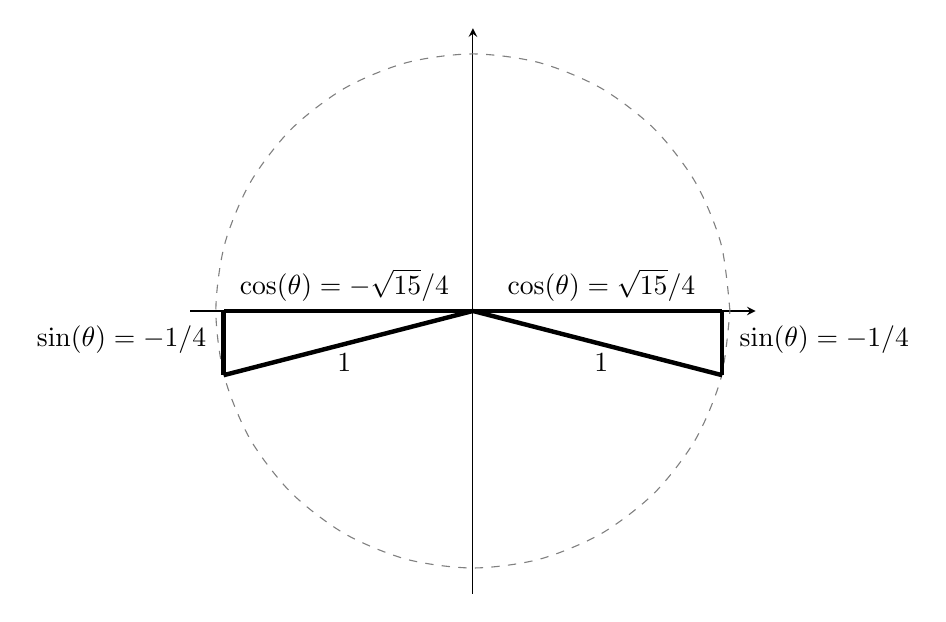
\begin{tikzpicture}
      \begin{axis}[
          xmin=-1.1,xmax=1.1,ymin=-1.1,ymax=1.1,
          axis lines=center,
          width=4in,
          ticks=none,
          clip=false,
          unit vector ratio*=1 1 1,
          %xlabel=$x$, ylabel=$y$,
          every axis y label/.style={at=(current axis.above origin),anchor=south},
          every axis x label/.style={at=(current axis.right of origin),anchor=west},
        ]        
        \addplot [black!50!white, dashed, smooth, domain=(0:360)] ({cos(x)},{sin(x)}); %% unit circle
        
        \addplot [ultra thick] plot coordinates {(0,0) (.97,-.25)}; 
        \addplot [ultra thick] plot coordinates {(.97,0) (.97,-.25)}; 
        \addplot [ultra thick] plot coordinates {(0,0) (.97,0)};

        \addplot [ultra thick] plot coordinates {(0,0) (-.97,-.25)}; 
        \addplot [ultra thick] plot coordinates {(-.97,0) (-.97,-.25)}; 
        \addplot [ultra thick] plot coordinates {(0,0) (-.97,0)}; 

        \node at (axis cs:-.5,-.2) {$1$};
        \node at (axis cs:.5,-.2) {$1$};
        \node[anchor=west] at (axis cs:1,-.11) {$\sin(\theta) = -1/4$};
        \node[anchor=east] at (axis cs:-1,-.11) {$\sin(\theta) = -1/4$};
        \node[anchor=south] at (axis cs:-.5,0) {$\cos(\theta) = -\sqrt{15}/4$};
        \node[anchor=south] at (axis cs:.5,0) {$\cos(\theta) = \sqrt{15}/4$};
        
      \end{axis}
    \end{tikzpicture}
  \end{image}
  Hence the derivative is zero at
  \begin{align*}
    x(\theta) &= \left(1+2\sin(\theta)\right)\cdot\cos(\theta)\\
    &= \left(1+2(-1/4)\right)\cdot \sqrt{15}/4\\
    &= \sqrt{15}/8,\\
    y(\theta) &= \left(1+2\sin(\theta)\right)\cdot\sin(\theta)\\
    &= \left(1+2(-1/4)\right)\cdot (-1/4)\\
    &= -1/8,
  \end{align*}
  meaning $(x,y) = (\sqrt{15}/8, -1/8)$, and
   \begin{align*}
    x(\theta) &= \left(1+2\sin(\theta)\right)\cdot\cos(\theta)\\
    &= \left(1+2(-1/4)\right)\cdot (-\sqrt{15}/4)\\
    &= -\sqrt{15}/8,\\
    y(\theta) &= \left(1+2\sin(\theta)\right)\cdot\sin(\theta)\\
    &= \left(1+2(-1/4)\right)\cdot (-1/4)\\
    &= -1/8,
  \end{align*}
   meaning $(x,y) = (-\sqrt{15}/8, -1/8)$.
\end{explanation}
\end{example}


  \begin{example}
Find Cartesian coordinates for where the graph of $r(\theta)
=1+2\sin(\theta)$ on $[0,2\pi]$ has vertical tangent lines.
\begin{explanation}
    To find the vertical lines of tangency, we set the denominator of
  $\frac{dy}{dx}=0$.
  \begin{align*}
    2(\cos^2\theta -\sin^2\theta)-\sin\theta &= 0 .
    \intertext{Convert the $\cos^2\theta$ term to $1-\sin^2\theta$:}
    2(1-\sin^2\theta-\sin^2\theta)-\sin\theta &= 0\\
    4\sin^2\theta + \sin\theta -1 &= 0.
  \end{align*}
  Recognize this as a quadratic in the variable $\sin\theta$. Using the quadratic formula, we have
  \begin{align*}
    \sin\theta &= \frac{-1\pm\sqrt{33}}{8}.
  \end{align*}
  We solve $\sin\theta = \frac{-1+\sqrt{33}}8$ and $\sin\theta = \frac{-1-\sqrt{33}}8$:
  \begin{align*}
    \sin\theta &=\frac{-1+\sqrt{33}}8 & \sin\theta &= \frac{-1-\sqrt{33}}{8}\\
    \theta &= \sin^{-1}\left(\frac{-1+\sqrt{33}}8\right) & \theta &= \sin^{-1}\left(\frac{-1-\sqrt{33}}8\right)\\
    \theta &= 0.6399 & \theta &= -1.0030
  \end{align*}
  In each of the solutions above, we only get one of the possible two solutions as $\sin^{-1}x$ only returns solutions in $[-\pi/2,\pi/2]$, the 4$^\text{th}$ and $1^\text{st}$ quadrants. Again using reference angles, we have:
  \[
  \sin\theta = \frac{-1+\sqrt{33}}8 \quad \Rightarrow \quad \theta = 0.6399,\ 3.7815 \text{ radians}
  \]
  and 
  \[
  \sin\theta = \frac{-1-\sqrt{33}}8 \quad \Rightarrow \quad \theta = 4.1446,\ 5.2802 \text{ radians.}
  \]
  These points are also shown in Figure \ref{fig:polcalc1} with
  white-filled dots.
\end{explanation}
\end{example}

\end{document}

%% }
%% {\begin{enumerate}
%% 	\item We start by computing $\frac{dy}{dx}$. With $\fp(\theta) = 2\cos\theta$, we have
%% 	\begin{align*}
%% 	\frac{dy}{dx} &= \frac{2\cos\theta\sin\theta + \cos\theta(1+2\sin\theta)}{2\cos^\theta-\sin\theta(1+2\sin\theta)}\\
%% 	&= \frac{\cos\theta(4\sin\theta+1)}{2(\cos^2\theta-\sin^2\theta)-\sin\theta}.
%% 	\end{align*}
%% 	When $\theta=\pi/4$, $\frac{dy}{dx}=-2\sqrt{2}-1$ (this requires a bit of simplification). In rectangular coordinates, the point on the graph at $\theta=\pi/4$ is $(1+\sqrt{2}/2,1+\sqrt{2}/2)$. Thus the rectangular equation of the line tangent to the lima\c con at $\theta=\pi/4$ is 
%% 	$$y=(-2\sqrt{2}-1)\big(x-(1+\sqrt{2}/2)\big)+1+\sqrt{2}/2 \approx  -3.83 x+8.24.$$ The lima\c con and the tangent line are graphed in Figure \ref{fig:polcalc1}. 
	
%% 	The normal line has the opposite--reciprocal slope as the tangent line, so its equation is 
%% 	$$y \approx \frac{1}{3.83}x+1.26.$$
%% 	\mfigure{.75}{The lima\c con in Example \ref{ex_polcalc1} with its tangent line at $\theta=\pi/4$ and points of vertical and horizontal tangency.}{fig:polcalc1}{figures/figpolcalc1}
%% 	\drawexampleline
	
%% 	\item		To find the horizontal lines of tangency, we find where $\frac{dy}{dx}=0$; thus we find where the numerator of our equation for $\frac{dy}{dx}$ is 0.
%% 	$$\cos\theta(4\sin\theta+1)=0\quad \Rightarrow \quad \cos\theta=0 \quad \text{or}\quad 4\sin\theta+1=0.$$
%% 	On $[0,2\pi]$, $\cos\theta=0$ when $\theta=\pi/2,\ 3\pi/2$. 

%% Setting $4\sin\theta+1=0$ gives $\theta=\sin^{-1}(-1/4)\approx -0.2527 = -14.48^\circ$. We want the results in $[0,2\pi]$; we also recognize there are two solutions, one in the 3$^\text{rd}$ quadrant and one in the 4$^\text{th}$. Using reference angles, we have our two solutions as $\theta =3.39$ and $6.03$ radians. The four points we obtained where the lima\c con has a horizontal tangent line are given in Figure \ref{fig:polcalc1} with black--filled dots.\\

%% To find the vertical lines of tangency, we set the denominator of $\frac{dy}{dx}=0$. 
%% \begin{align*}
%% 2(\cos^2\theta -\sin^2\theta)-\sin\theta &= 0 .
%% \intertext{Convert the $\cos^2\theta$ term to $1-\sin^2\theta$:}
%% 2(1-\sin^2\theta-\sin^2\theta)-\sin\theta &= 0\\
%% 4\sin^2\theta + \sin\theta -1 &= 0.
%% \intertext{Recognize this as a quadratic in the variable $\sin\theta$. Using the quadratic formula, we have}
%% \sin\theta &= \frac{-1\pm\sqrt{33}}{8}.
%% \end{align*}
%% We solve $\sin\theta = \frac{-1+\sqrt{33}}8$ and $\sin\theta = \frac{-1-\sqrt{33}}8$:
%% \begin{align*}
%% \sin\theta &=\frac{-1+\sqrt{33}}8 & \sin\theta &= \frac{-1-\sqrt{33}}{8}\\
%% \theta &= \sin^{-1}\left(\frac{-1+\sqrt{33}}8\right) & \theta &= \sin^{-1}\left(\frac{-1-\sqrt{33}}8\right)\\
%% \theta &= 0.6399 & \theta &= -1.0030
%% \end{align*}
%% In each of the solutions above, we only get one of the possible two solutions as $\sin^{-1}x$ only returns solutions in $[-\pi/2,\pi/2]$, the 4$^\text{th}$ and $1^\text{st}$ quadrants. Again using reference angles, we have:
%% $$\sin\theta = \frac{-1+\sqrt{33}}8 \quad \Rightarrow \quad \theta = 0.6399,\ 3.7815 \text{ radians}$$
%% and 
%% $$\sin\theta = \frac{-1-\sqrt{33}}8 \quad \Rightarrow \quad \theta = 4.1446,\ 5.2802 \text{ radians.}$$
%% These points are also shown in Figure \ref{fig:polcalc1} with white--filled dots.
%% 	\end{enumerate}
%% 	\vskip-\baselineskip
%% }\\

%% When the graph of the polar function $r=f(\theta)$ intersects the pole, it means that $f(\alpha)=0$ for some angle $\alpha$. Thus the formula for $\frac{dy}{dx}$ in such instances is very simple, reducing simply to $$\frac{dy}{dx} = \tan \alpha.$$
%% This equation makes an interesting point. It tells us the slope of the tangent line at the pole is $\tan \alpha$; some of our previous work (see, for instance, Example \ref{ex_polar3}) shows us that the line through the pole with slope $\tan \alpha$ has polar equation $\theta=\alpha$. Thus when a polar graph touches the pole at $\theta=\alpha$, the equation of the tangent line at the pole is $\theta=\alpha$. \\

%% \example{ex_polcalc2}{Finding tangent lines at the pole.}{
%% Let $r=1+2\sin\theta$, a lima\c con. Find the equations of the lines tangent to the graph at the pole.
%% \mfigure{.35}{Graphing the tangent lines at the pole in Example \ref{ex_polcalc2}.}{fig:polcalc2}{figures/figpolcalc2}}
%% {We need to know when $r=0$. 
%% \begin{align*}
%% 1+2\sin\theta &= 0\\
%% \sin\theta &= -1/2\\
%% \theta &= \frac{7\pi}{6},\ \frac{11\pi}6.
%% \end{align*}
%% Thus the equations of the tangent lines, in polar, are $\theta = 7\pi/6$ and $\theta = 11\pi/6$. In rectangular form, the tangent lines are $y=\tan(7\pi/6)x$ and $y=\tan(11\pi/6)x$. The full lima\c con can be seen in Figure \ref{fig:polcalc1}; we zoom in on the tangent lines in Figure \ref{fig:polcalc2}.
%% }\\
















